\section{Modifying and applying RISE (Single Pixel)}
\nblink{brats/06\_rise.ipynb}

apply on a single pixel, pixel == class

\subsection{Results}

\begin{figure}[H]
\centering
\caption{Extracted horizontal slices with merged tumor segment}
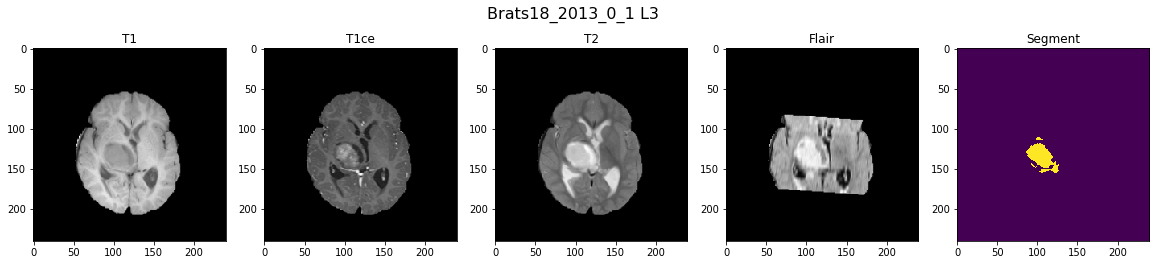
\includegraphics[width=15cm]{chapters/04_segmentation/images/preprocessing.png}
\end{figure}



\subsection{Discussion}

\subsection{Conclusion}
Works, but low resolution even with 3000 masks

\section{Modifying and applying RISE (Multi Pixel)}
\nblink{17\_rise\_multipixel.ipynb}


\begin{figure}[H]
\centering
\caption{RISE Multipixel (Mean)}
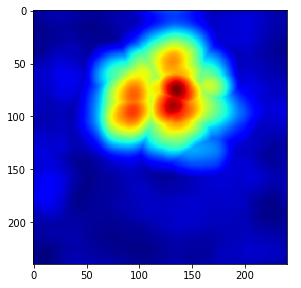
\includegraphics[width=5cm]{chapters/04_segmentation/images/rise_multipixel_max_1-0.png}
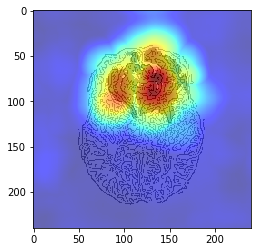
\includegraphics[width=5cm]{chapters/04_segmentation/images/rise_multipixel_max_1-1.png}
\end{figure}




\subsection{Results}

\subsection{Discussion}

\subsection{Conclusion}
